\documentclass[aspectratio=169,10pt,dvipsnames,xcolor=table,handout]{beamer}

%\setbeameroption{show notes}

\input{preamble.inc}

\title{Reti logiche}

\begin{document}

\begin{frame}
    \titlepage
\end{frame}

\begin{frame}{Logica e progettazione di calcolatori}
    Questa lezione è un po' una digressione rispetto all'argomento principale del corso, ma ritengo interessante vedere come i concetti della logica si utilizzano in ambiti applicativi completamente diversi.

    \medskip
    Vedremo come le CPU in buona parte implementano delle enormi formule logiche in cui però ``vero'' e ``falso'' sono rimpiazzati da presenza e assenza di corrente.
\end{frame}

\section{Dalle operazioni numeriche alla logica}

\begin{frame}{Sommare tre cifre binarie (1)}
    Tra le operazioni che la CPU deve fare, una ovviamente è la somma di numeri.

    \medskip
    Supponiamo di dover costruire un circuito che esegue la somma di tre cifre binarie. L'output sarà numero di due bit. Questo circuito prende il nome di \alert{sommatore completo}.

    \medskip
    Questa tabella mostra l'output prodotto dal circuito per ogni possibile input:
    \begin{center}
        \begin{tabular}{|c|c|c||c|}
            $a$ & $b$ & $c$ & $a+b+c$ \\
            \hline
            0   & 0   & 0   & 00 (0)  \\
            0   & 0   & 1   & 01 (1)  \\
            0   & 1   & 0   & 01 (1)  \\
            0   & 1   & 1   & 10 (2)  \\
            1   & 0   & 0   & 01 (1)  \\
            1   & 0   & 1   & 10 (2)  \\
            1   & 1   & 0   & 10 (2)  \\
            1   & 1   &ù 1   & 11 (3)  \\
        \end{tabular}
    \end{center}
\end{frame}

\begin{frame}{Sommare tre cifre binarie (2)}
    \begin{center}
        \only<1-2>{
            \begin{tabular}{|c|c|c||c|}
                $a$ & $b$ & $c$ & $a+b+c$ \\
                \hline
                0   & 0   & 0   & 00 (0)  \\
                0   & 0   & 1   & 01 (1)  \\
                0   & 1   & 0   & 01 (1)  \\
                0   & 1   & 1   & 10 (2)  \\
                1   & 0   & 0   & 01 (1)  \\
                1   & 0   & 1   & 10 (2)  \\
                1   & 1   & 0   & 10 (2)  \\
                1   & 1   & 1   & 11 (3)  \\
            \end{tabular}}%
        \only<3-4>{
            \begin{tabular}{|c|c|c||c|c|}
                $a$ & $b$ & $c$ & $r$ & $s$ \\
                \hline
                0   & 0   & 0   & 0   & 0   \\
                0   & 0   & 1   & 0   & 1   \\
                0   & 1   & 0   & 0   & 1   \\
                0   & 1   & 1   & 1   & 0   \\
                1   & 0   & 0   & 0   & 1   \\
                1   & 0   & 1   & 1   & 0   \\
                1   & 1   & 0   & 1   & 0   \\
                1   & 1   & 1   & 1   & 1   \\
            \end{tabular}
        }%
        \only<5>{
            \begin{tabular}{|c|c|c||c|c|}
                $A$ & $B$ & $C$ & $R$ & $S$ \\
                \hline
                F   & F   & F   & F   & F   \\
                F   & F   & V   & F   & V   \\
                F   & V   & F   & F   & V   \\
                F   & V   & V   & V   & F   \\
                V   & F   & F   & F   & V   \\
                V   & F   & V   & V   & F   \\
                V   & V   & F   & V   & F   \\
                V   & V   & V   & V   & V   \\
            \end{tabular}
        }%
    \end{center}

    \medskip
    Partendo da questa tabella:
    \begin{itemize}
        \item<2-> Separiamo le due cifre binarie dell'output in due colonne
        \item<4-> Rimiazziamo 0 ed 1 con V ed F
    \end{itemize}
    \uncover<5->{Ottieniamo una tabella di verità per due funzioni proposizionali $R$ e $S$}
\end{frame}

\begin{frame}{Formule logiche del sommatore}
    Usando tecniche già viste, possiamo ricavare le forme proposizionali per le colonne $R$ ed $S$, che sono:
    \begin{itemize}
        \item $R = \begin{array}[t]{l}
            (\lnot A \land B \land C) \lor (A \land \lnot B \land C) \lor (A \land B \land \lnot C) \lor (A \land B \land C) \\
            \equiv (B \wedge C) \vee (A \wedge (B \vee C))
        \end{array}$
        \item $S = \begin{array}[t]{l}
            (\lnot A \land B \land \lnot C) \lor (A \land \lnot B \land C) \lor (A \land \lnot B \land \not C) \lor (A \land B \land C) \\
            \equiv A \xor B \xor C
        \end{array}$
    \end{itemize}

    \smallskip
    Per curiosità, si noti che una disgiunzione esclusiva tra più lettere proposizionali, come $A \xor B \xor C$, è vera quando il numero di lettere che hanno valore di verità vero è dispari.

    \medskip
    Abbiamo quindi due formle logiche che ``implementano''  le operazioni di somma di tre numeri a un bit.
\end{frame}

\begin{frame}{Dalla somma di bit alla somma di numeri (1)}
    Possiamo schematizzare il sommatore completo in questo modo:
    \begin{center}
        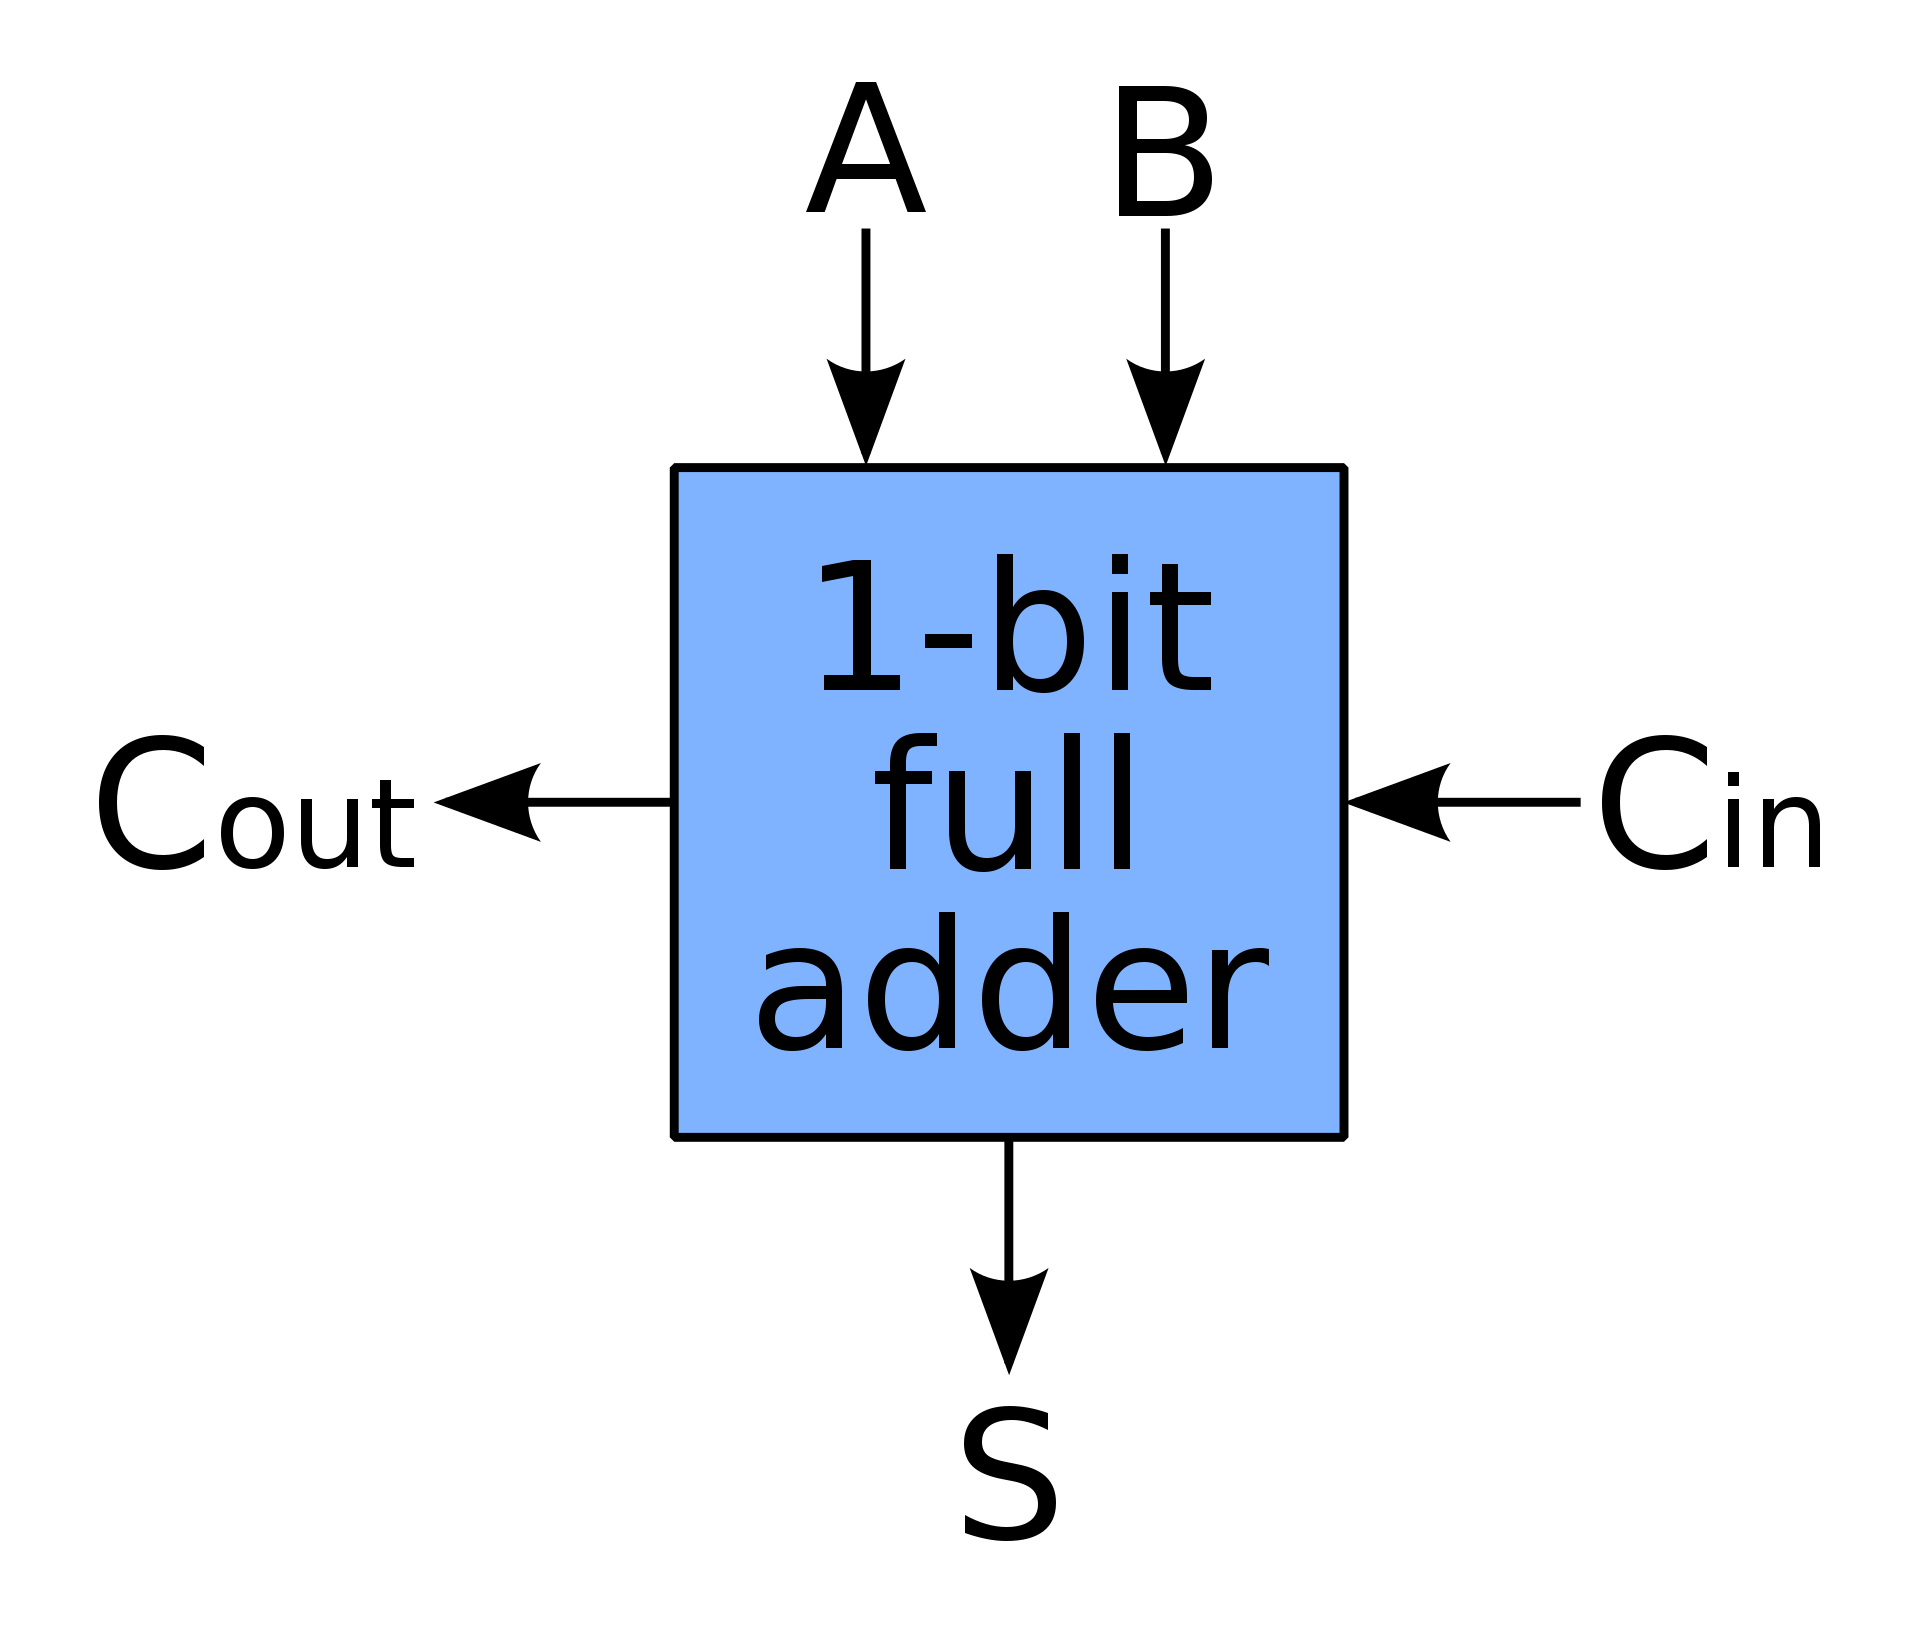
\includegraphics[height=0.3\textheight]{1-bit_full-adder.png}
    \end{center}
    \begin{itemize}
        \item $A$, $B$, e $C_{in}$ sono i bit da sommare;
        \item $S$ e $C_{out}$ sono il risultato. In particolare:
        \begin{itemize}
            \item $S$ è il bit meno significativo del risultato;
            \item $C_{out}$ è il bit più significativo del risultato, chiamato \emph{riporto} (o \emph{carry} in inglese).
        \end{itemize}
    \end{itemize}
    \vfill
    {\scriptsize  Immagine \copyright\ en:User:Cburnett - Own work, CC BY-SA 3.0, \url{https://commons.wikimedia.org/w/index.php?curid=1477628}}
\end{frame}

\begin{frame}{Dalla somma di bit alla somma di numeri (2)}
    Come si sommano due numeri in colonna (in base 2 o 10 che sia) ?
    \begin{itemize}
        \item Si sommano prima le unità. Siccome la somma può dare come risultato un numero con due cifre, si scrive la cifra delle unità e si tiene da parte la cifra delle decine (che si chiama \emph{riporto}).
        \item Si passa quindi alle cifra a sinistra: queste si sommano tra di loro e assieme al riporto generato al passo prima. Il risultato di questa somma è anch'esso costituito da una cifra di risultato ed una di riporto.
        \item E così via per le cifre ancora più significative.
    \end{itemize}
    Seguendo questo principio, se dobbiamo sommare due numeri composti da vari bit, possiamo collegare in cascata vari circuiti addizionatori.
\end{frame}

\begin{frame}{Dalla somma di bit alla somma di numeri (3)}
    Ad esempio, se abbiamo due numeri di 4 cifre ($A_3 A_2 A_1 A_0$ e $B_3 B_2 B_1 B_0$) un circuito che li somma si può ottenere come segue:
    \begin{center}
        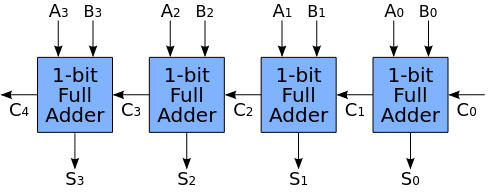
\includegraphics[height=0.3\textheight]{4-bit_adder.png}
    \end{center}
    Il risultato è costituito da $S_3 S_2 S_1 S_0$ con il riporto $C_4$. L'input $C_0$ è il riporto da una eventuale addizione precedente, che può essere posto a 0 / falso se non c'è nessun riporto da considerare.
    \vfill
    {\scriptsize Immagine \copyright\ en:User:Cburnett - This W3C-unspecified vector image was created with Inkscape ., CC BY-SA 3.0, \url{https://commons.wikimedia.org/w/index.php?curid=1477488}}
\end{frame}


\section{Dalla logica ai circuiti elettrici}

\begin{frame}{Interruttori elettronici}
    Per ora questi circuiti sono comunque oggeti puramente logico/matematici. Come si fa a costruire un circuito che implementa effettivamente una formula logica?
    \begin{itemize}
        \item si associa un livello di tensione ai due valori di verità: ad esempio, 0 Volt per il valore falso e 5 Volt per il valore vero;
        \item si utilizzano degli \alert{interruttori elettronici}, ovvero degli interruttori concettualmente simili a quelli che usiamo per accendere la luce, ma che si possono aprire e chiudere tramite un segnale elettrico.

        \medskip
        La tecnologia degli interrutori elettronici è cambiata nel tempo:
        \begin{itemize}
            \item relè
            \item valvole termoioniche
            \item diodi
            \item transistor
        \end{itemize}
    \end{itemize}
\end{frame}

\begin{frame}{Il connettivo AND}
    Ecco come realizzare il connettivo AND con una coppia di transistor:
    \begin{center}
        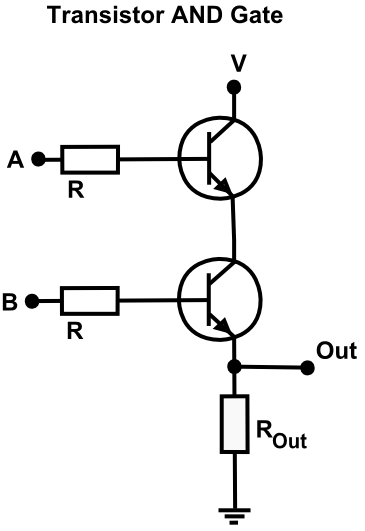
\includegraphics[height=0.5\textheight]{TransistorANDgate.png}
    \end{center}
    \begin{itemize}
        \item se $A$ e $B$ sono entrambi veri, i due transistor fanno passare la corrente, e nel punto \textit{Out} si misura la tensione $V$ (+5 V);
        \item appena uno solo tra $A$ o $B$ è falso (0 V), il transistor scollega il circuito, e nel punto \textit{Out} si misura 0 V.
    \end{itemize}
\end{frame}

\begin{frame}{VLSI}
    I pezzi che compongono il circuito di sopra si possono acquistare uno per uno. Ma ovviamente così anche un semplice sommatore diventa gigantesco.

    \medskip
    Col tempo, si è imparato a costruire \emph{circuiti integrati} che contengono miliardi di transistor. Questa tecnologia prende il nome di \alert{VLSI} (Very Large Scale Integration).

    \medskip
    Ad esempio:
    \begin{itemize}
        \item la CPU Apple M2 che si trova sui nuovo Mac ha circa 20 miliardi di transistor;
        \item la GPU nVidia GTX 3090 ha circa 28.3 miliardi di transistor.
    \end{itemize}

    \medskip
    Empiricamente, si è visto che il numero di transistor che si riesce a inserire in un unico circuito integrato raddoppia ogni due anni. Questa evidenza empirica è nota come \alert{legge di Moore}.

    \medskip
    Sembra però che la legge di Moore stia per arrivare al suo limite.
\end{frame}

\begin{frame}{La legge di Moore}
    \centering
    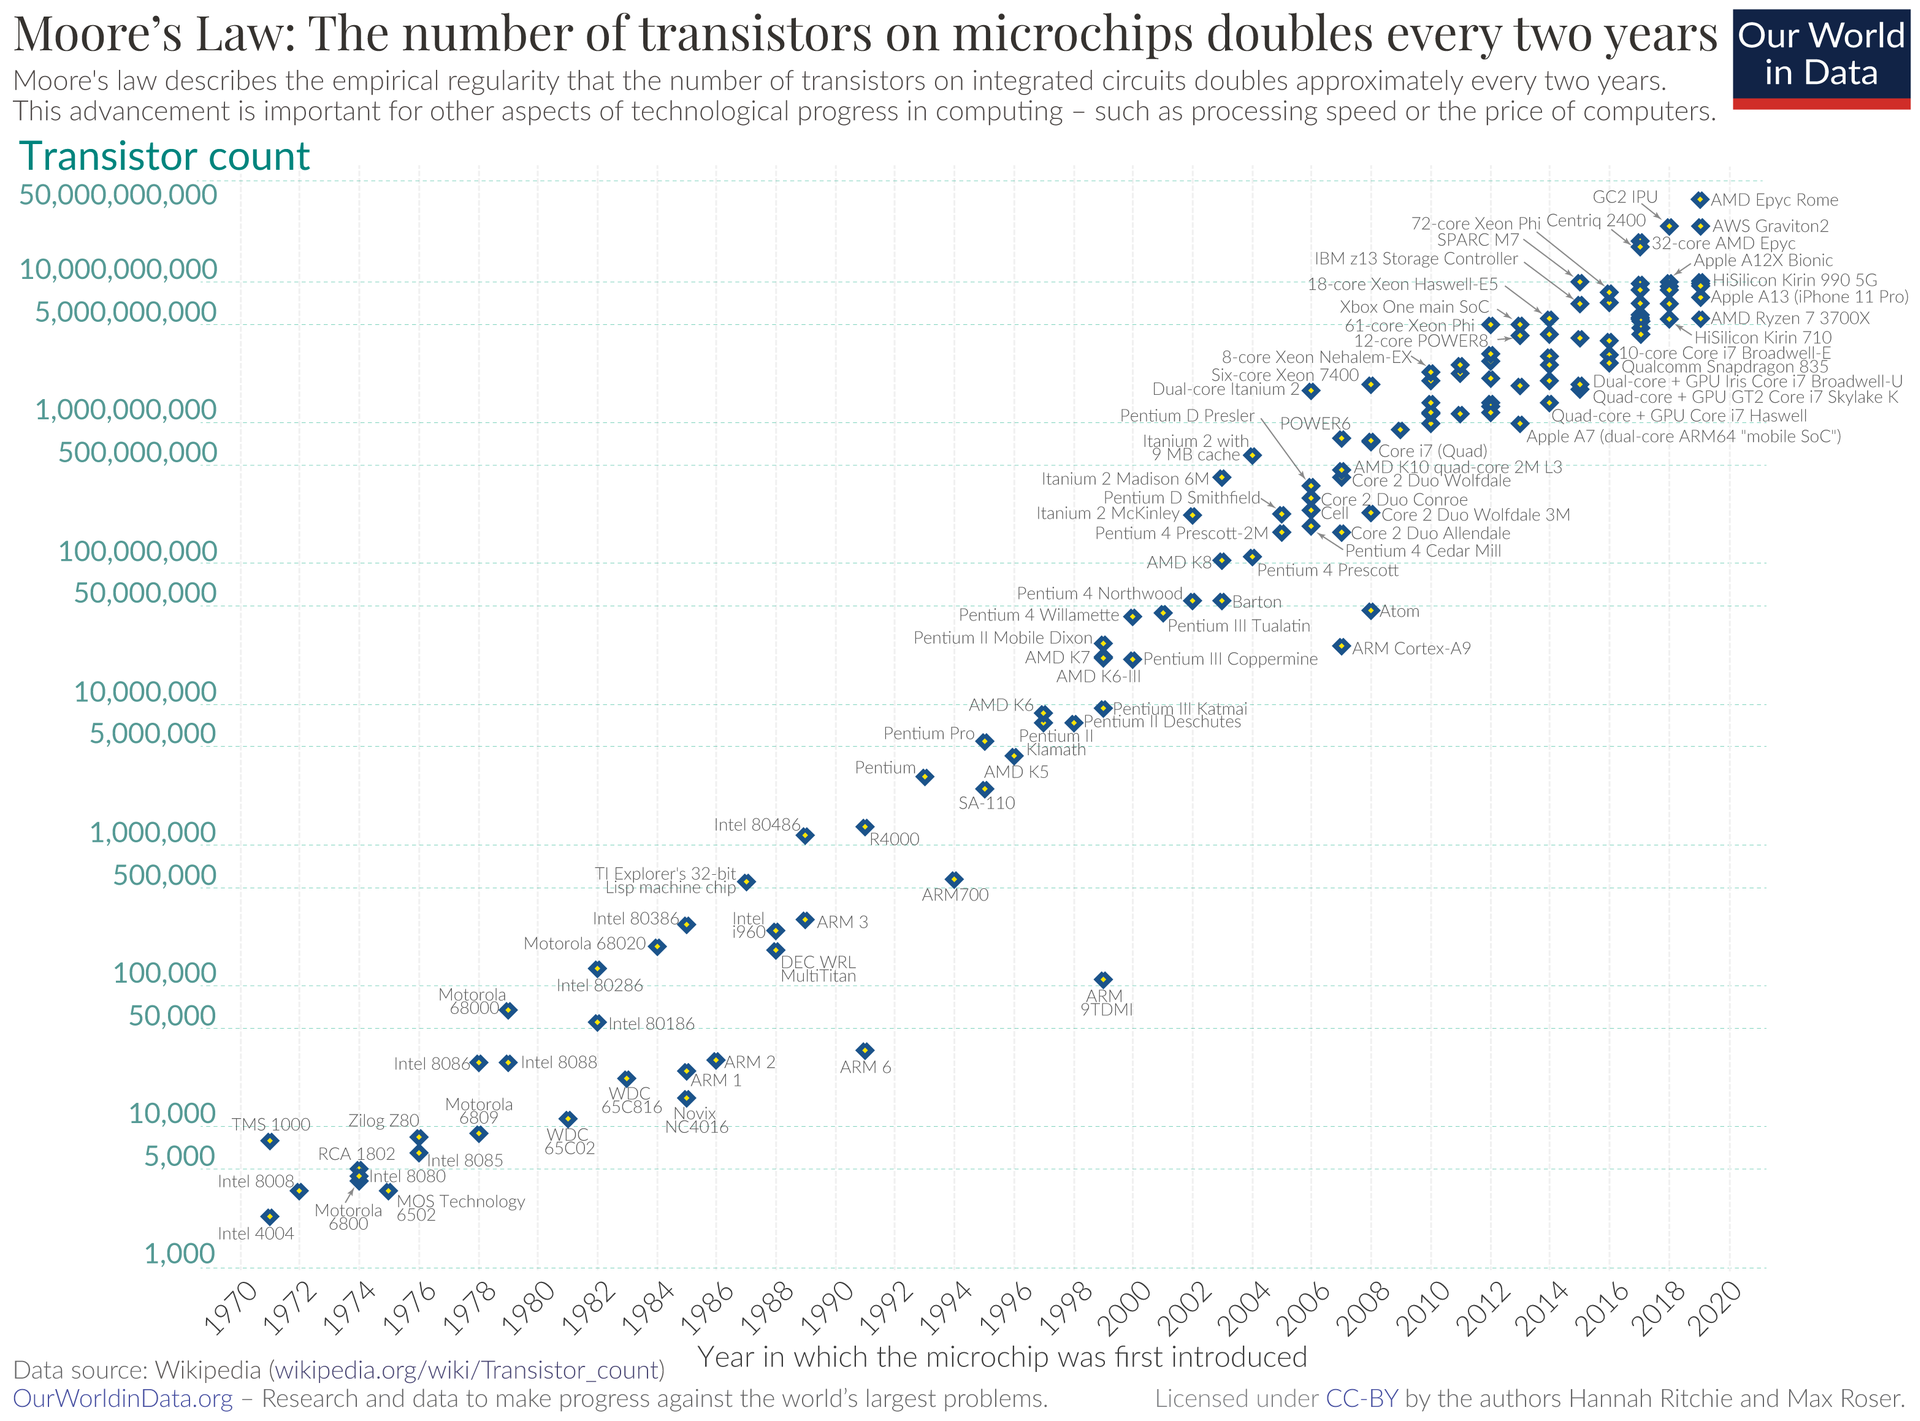
\includegraphics[height=0.95\textheight]{Moore's_Law_Transistor_Count_1970-2020.png}
\end{frame}
\end{document}